\documentclass[tikz,border=3pt]{standalone}
\usetikzlibrary{arrows.meta,positioning,calc,fit}
\definecolor{esrblue}{RGB}{34,91,151}
\definecolor{caporange}{RGB}{190,92,20}
\definecolor{gategray}{RGB}{90,96,105}
\begin{document}
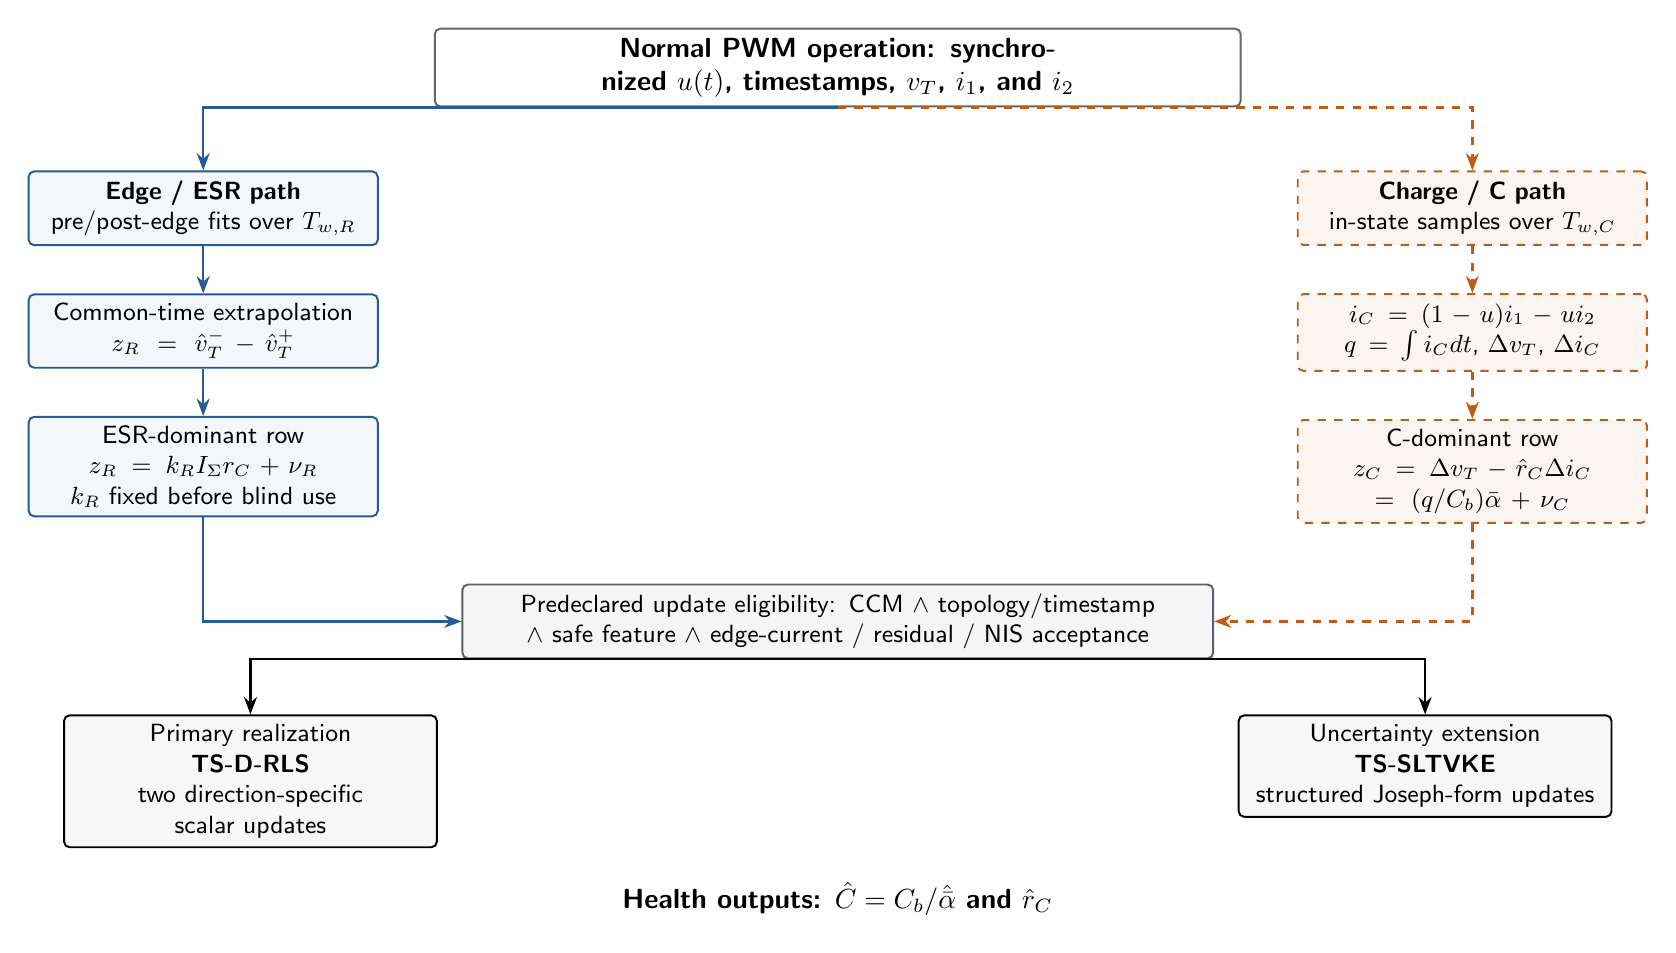
\begin{tikzpicture}[
  font=\sffamily\small,
  block/.style={rounded corners=2pt,draw=black!60,fill=white,align=center,
    minimum height=8mm,text width=42mm,line width=0.7pt},
  esr/.style={block,draw=esrblue,fill=esrblue!5},
  cpath/.style={block,draw=caporange,fill=caporange!6,dashed},
  gate/.style={block,draw=gategray,fill=black!4,text width=93mm},
  output/.style={block,draw=black,fill=black!3,text width=45mm},
  arr/.style={-{Stealth[length=2.2mm]},line width=0.85pt},
  esrarr/.style={arr,draw=esrblue},
  caparr/.style={arr,draw=caporange,dashed}]

  \node[block,text width=100mm,font=\sffamily\bfseries] (sync)
    {Normal PWM operation: synchronized $u(t)$, timestamps, $v_T$, $i_1$, and $i_2$};

  \node[esr,below left=8mm and 7mm of sync] (esr1)
    {\textbf{Edge / ESR path}\\pre/post-edge fits over $T_{w,R}$};
  \node[cpath,below right=8mm and 7mm of sync] (cap1)
    {\textbf{Charge / C path}\\in-state samples over $T_{w,C}$};
  \draw[esrarr] (sync.south) -| (esr1.north);
  \draw[caparr] (sync.south) -| (cap1.north);

  \node[esr,below=6mm of esr1] (esr2)
    {Common-time extrapolation\\$z_R=\hat v_T^- -\hat v_T^+$};
  \node[cpath,below=6mm of cap1] (cap2)
    {$i_C=(1-u)i_1-ui_2$\\$q=\int i_Cdt$, $\Delta v_T$, $\Delta i_C$};
  \draw[esrarr] (esr1) -- (esr2);
  \draw[caparr] (cap1) -- (cap2);

  \node[esr,below=6mm of esr2] (esr3)
    {ESR-dominant row\\$z_R=k_RI_\Sigma r_C+\nu_R$\\$k_R$ fixed before blind use};
  \node[cpath,below=6mm of cap2] (cap3)
    {C-dominant row\\$z_C=\Delta v_T-\hat r_C\Delta i_C$\\$=(q/C_b)\bar\alpha+\nu_C$};
  \draw[esrarr] (esr2) -- (esr3);
  \draw[caparr] (cap2) -- (cap3);

  \node[gate,below=8mm of $(esr3.south)!0.5!(cap3.south)$] (gates)
    {Predeclared update eligibility: CCM $\land$ topology/timestamp
     $\land$ safe feature $\land$ edge-current / residual / NIS acceptance};
  \draw[esrarr] (esr3) |- (gates.west);
  \draw[caparr] (cap3) |- (gates.east);

  \node[output,below left=7mm and 3mm of gates] (rls)
    {Primary realization\\\textbf{TS-D-RLS}\\two direction-specific scalar updates};
  \node[output,below right=7mm and 3mm of gates] (kf)
    {Uncertainty extension\\\textbf{TS-SLTVKE}\\structured Joseph-form updates};
  \draw[arr] (gates.south) -| (rls.north);
  \draw[arr] (gates.south) -| (kf.north);

  \node[below=5mm of $(rls.south)!0.5!(kf.south)$,align=center,font=\sffamily\bfseries]
    {Health outputs: $\hat C=C_b/\hat{\bar\alpha}$ and $\hat r_C$};

\end{tikzpicture}
\end{document}
